%\documentclass[11pt,epsf]{article}
\documentclass[oneside, a4paper, onecolumn, 11pt]{article}

\usepackage{graphicx, amssymb, multicol, amsmath}
\usepackage{fancyhdr, hyperref, sidecap}
%\usepackage[left=2.05cm,top=2.05cm,bottom=1.55cm,right=2.05cm]{geometry}
\usepackage[left=2.05cm,top=2.05cm,right=2.05cm]{geometry}
\usepackage[utf8]{inputenc}
\usepackage{natbib}	        %%  bibliography style
\setlength{\bibsep}{0.0pt}
\usepackage{eurosym}
\usepackage{enumitem}
\usepackage{nopageno}
\usepackage{fancyhdr}
\usepackage[usenames,dvipsnames,svgnames,table]{xcolor}

\usepackage{amsmath, amssymb}
\usepackage{booktabs, bm}           %%  bold math
\usepackage{cancel}
\usepackage{dcolumn}  %%  Align table columns on decimal point
\usepackage{epsfig, epsf, eurosym, enumitem}
\usepackage{fancyhdr}
\usepackage[T1]{fontenc}
\usepackage[para]{footmisc}
\usepackage{graphicx }
%\usepackage{lscape}
\usepackage{hyperref,ifthen}
\usepackage{mathptmx, multicol}
\usepackage[authoryear, round]{natbib}
\usepackage{nopageno}
\usepackage{subfigure}
\usepackage{verbatim}
\usepackage{threeparttable}
\usepackage[usenames,dvipsnames]{xcolor}
\usepackage{tcolorbox}
\usepackage{tabularx}
\usepackage{array}
\usepackage{colortbl}
\usepackage{framed}
\usepackage{todonotes}



%%%%%%%%%%%%%%%%%%%%%%%%%%%%%%%%%%%%%%%%%%%
%       define Journal abbreviations      %
%%%%%%%%%%%%%%%%%%%%%%%%%%%%%%%%%%%%%%%%%%%
\def\nat{Nat} \def\apjl{ApJ~Lett.} \def\apj{ApJ}
\def\apjs{ApJS} \def\aj{AJ} \def\mnras{MNRAS}
\def\prd{Phys.~Rev.~D} \def\prl{Phys.~Rev.~Lett.}
\def\plb{Phys.~Lett.~B} \def\jhep{JHEP}
\def\npbps{NUC.~Phys.~B~Proc.~Suppl.} \def\prep{Phys.~Rep.}
\def\pasp{PASP} \def\aap{Astron.~\&~Astrophys.} \def\araa{ARA\&A}
\def\jcap{\ref@jnl{J. Cosmology Astropart. Phys.}} 
\def\nar{New~A.R.} \def\aapr{A\&ARv}

\newcommand{\preep}[1]{{\tt #1} }

%%%%%%%%%%%%%%%%%%%%%%%%%%%%%%%%%%%%%%%%%%%%%%%%%%%%%
%              define symbols                       %
%%%%%%%%%%%%%%%%%%%%%%%%%%%%%%%%%%%%%%%%%%%%%%%%%%%%%
\def \Mpc {~{\rm Mpc} }
\def \Om {\Omega_0}
\def \Omb {\Omega_{\rm b}}
\def \Omcdm {\Omega_{\rm CDM}}
\def \Omlam {\Omega_{\Lambda}}
\def \Omm {\Omega_{\rm m}}
\def \ho {H_0}
\def \qo {q_0}
\def \lo {\lambda_0}
\def \kms {{\rm ~km~s}^{-1}}
\def \kmsmpc {{\rm ~km~s}^{-1}~{\rm Mpc}^{-1}}
\def \hmpc{~\;h^{-1}~{\rm Mpc}} 
\def \hkpc{\;h^{-1}{\rm kpc}} 
\def \hmpcb{h^{-1}{\rm Mpc}}
\def \dif {{\rm d}}
\def \mlim {m_{\rm l}}
\def \bj {b_{\rm J}}
\def \mb {M_{\rm b_{\rm J}}}
\def \mg {M_{\rm g}}
\def \mi {M_{\rm i}}
\def \qso {_{\rm QSO}}
\def \lrg {_{\rm LRG}}
\def \gal {_{\rm gal}}
\def \xibar {\bar{\xi}}
\def \xis{\xi(s)}
\def \xisp{\xi(\sigma, \pi)}
\def \Xisig{\Xi(\sigma)}
\def \xir{\xi(r)}
\def \max {_{\rm max}}
\def \gsim { \lower .75ex \hbox{$\sim$} \llap{\raise .27ex \hbox{$>$}} }
\def \lsim { \lower .75ex \hbox{$\sim$} \llap{\raise .27ex \hbox{$<$}} }
\def \deg {^{\circ}}
%\def \sqdeg {\rm deg^{-2}}
\def \deltac {\delta_{\rm c}}
\def \mmin {M_{\rm min}}
\def \mbh  {M_{\rm BH}}
\def \mdh  {M_{\rm DH}}
\def \msun {M_{\odot}}
\def \z {_{\rm z}}
\def \edd {_{\rm Edd}}
\def \lin {_{\rm lin}}
\def \nonlin {_{\rm non-lin}}
\def \wrms {\langle w_{\rm z}^2\rangle^{1/2}}
\def \dc {\delta_{\rm c}}
\def \wp {w_{p}(\sigma)}
\def \PwrSp {\mathcal{P}(k)}
\def \DelSq {$\Delta^{2}(k)$}
\def \WMAP {{\it WMAP \,}}
\def \cobe {{\it COBE }}
\def \COBE {{\it COBE \;}}
\def \HST  {{\it HST \,\,}}
\def \Spitzer  {{\it Spitzer \,}}
\def \ATLAS {VST-AA$\Omega$ {\it ATLAS} }
\def \BEST   {{\tt best} }
\def \TARGET {{\tt target} }
\def \TQSO   {{\tt TARGET\_QSO}}
\def \HIZ    {{\tt TARGET\_HIZ}}
\def \FIRST  {{\tt TARGET\_FIRST}}
\def \zc {z_{\rm c}}
\def \zcz {z_{\rm c,0}}


\newcommand{\sqdeg}{deg$^{-2}$}
\newcommand{\lya}{Ly$\alpha$\ }
%\newcommand{\lya}{Ly\,$\alpha$\ }
\newcommand{\lyaf}{Ly\,$\alpha$\ forest}
%\newcommand{\eg}{e.g.~}
%\newcommand{\etal}{et~al.~}
\newcommand{\cii}{C\,{\sc ii}\ }
\newcommand{\ciii}{C\,{\sc iii}]\ }
\newcommand{\civ}{C\,{\sc iv}\ }
\newcommand{\SiIV}{Si\,{\sc iv}\ }
\newcommand{\mgii}{Mg\,{\sc ii}\ }
\newcommand{\feii}{Fe\,{\sc ii}\ }
\newcommand{\feiii}{Fe\,{\sc iii}\ }
\newcommand{\caii}{Ca\,{\sc ii}\ }
\newcommand{\halpha}{H\,$\alpha$\ }
\newcommand{\hbeta}{H\,$\beta$\ }
\newcommand{\oi}{[O\,{\sc i}]\ }
\newcommand{\oii}{[O\,{\sc ii}]\ }
\newcommand{\oiii}{[O\,{\sc iii}]\ }
\newcommand{\heii}{[He\,{\sc ii}]\ }
\newcommand{\nii}{N\,{\sc ii}\ }
\newcommand{\nv}{N\,{\sc v}\ }

%% From:: /cos_pc19a_npr/LaTeX/proposals/JWST/JWST_ERS/Proposal/lines.tex
%%  
\newcommand{\imw}{$i$--$W3$}
\newcommand{\imwf}{$i$--$W4$}
\newcommand{\rmwf}{$r$--$W4$}
\newcommand{\imwt}{$i$--$W2$}
\newcommand{\wtmwf}{$W3$--$W4$}
%\newcommand{\kms}{km s$^{-1}$}
\newcommand{\cmN}{cm$^{-2}$}
\newcommand{\cmn}{cm$^{-3}$}
%\newcommand{\msun}{M$_{\odot}$}
\newcommand{\lsun}{L$_{\odot}$}
\newcommand{\lam}{$\lambda$}
\newcommand{\mum}{$\mu$m}
\newcommand{\ebv}{$E(B$$-$$V)$}
%\newcommand{\heii}{\mbox{He\,{\sc ii}}}
\newcommand{\cv}{\mbox{C\,{\sc v}}}
%\newcommand{\civ}{\mbox{C\,{\sc iv}}}
%\newcommand{\ciii}{\mbox{C\,{\sc iii}}}
%\newcommand{\cii}{\mbox{C\,{\sc ii}}}
%\newcommand{\nv}{\mbox{N\,{\sc v}}}
\newcommand{\niv}{\mbox{N\,{\sc iv}}}
\newcommand{\niii}{\mbox{N\,{\sc iii}}}
%\newcommand{\oi}{\mbox{O\,{\sc i}}}
%\newcommand{\oii}{\mbox{O\,{\sc ii}}}
%\newcommand{\oiii}{\mbox{[O\,{\sc iii}]}}
\newcommand{\oiv}{\mbox{O\,{\sc iv}}}
\newcommand{\ov}{\mbox{O\,{\sc v}}}
\newcommand{\ovi}{\mbox{O\,{\sc vi}}}
\newcommand{\ovii}{\mbox{O\,{\sc vii}}}

%\newcommand{\feii}{\mbox{Fe\,{\sc ii}}}
%\newcommand{\feiii}{\mbox{Fe\,{\sc iii}}}
%\newcommand{\mgii}{\mbox{Mg\,{\sc ii}}}
\newcommand{\neii}{[Ne\,{\sc ii}]\ }
\newcommand{\neiii}{[Ne\,{\sc ii}]\ }
\newcommand{\nev}{Ne\,{\sc v}\ }
\newcommand{\nevi}{[Ne\,{\sc vi}]\ }
\newcommand{\neviii}{\mbox{Ne\,{\sc viii}}}
\newcommand{\aliii}{\mbox{Al\,{\sc iii}}}
\newcommand{\siii}{\mbox{Si\,{\sc ii}}}
\newcommand{\siiii}{\mbox{Si\,{\sc iii}}}
\newcommand{\siiv}{\mbox{Si\,{\sc iv}}}
%\newcommand{\lya}{\mbox{Ly$\alpha$}}
%\newcommand{\lyb}{\mbox{Ly$\beta$}}
\newcommand{\hi}{\mbox{H\,{\sc i}}}
\newcommand{\snine}{\mbox{[S\,{\sc ix}]}}
\newcommand{\sivi}{\mbox{[Si\,{\sc vi}]}}
\newcommand{\sivii}{\mbox[{Si\,{\sc vii}]}}
\newcommand{\siix}{\mbox{[Si\,{\sc ix}]}}
\newcommand{\six}{\mbox{[Si\,{\sc x}]}}
\newcommand{\sixi}{\mbox{[Si\,{\sc xi}]}}
\newcommand{\caviii}{\mbox{[Ca\,{\sc viii}]}}
\newcommand{\arii}{\mbox{[Ar\,{\sc ii}]}}

%%[Ar II] 6.97
%% [S IX] 1.252 μm 328 
% [Si X] 1.430 μm 351 
% [Si XI] 1.932 μm 401 
% [Si VI] 1.962 μm 167 
% [Ca VIII] 2.321 μm 128 
% [Si VII] 2.483 μm 205 
% [Si IX] 3.935 μm 303
% [Ar II] 6.97


%\snine\ at 1.252$\mu$m, \six\ at 1.430$\mu$m, \sixi\ at 1.932$\mu$m, \sivi\ at
%1.962$\mu$m, \caviii\ at 2.321$\mu$m, \sivi\ at 2.483$\mu$m \siix\ at
%3.935$\mu$m and \arii\ at 6.97$\mu$m. 
%%
%% such as [Ne ii]12.8 μm, [Ne v]14.3 μm, [Ne iii]15.5 μm, [S iii]18.7 μm and 33.48 μm, [O iv]25.89 μm and [Si ii]34.8 μm (e.g
%%
%% MIR emission lines like [NeII] and [NeV] are ..
%%
%% Also,  arXiv:astro-ph/0003457v1 
%% [NeV] 14.32um & 24.32um and [NeVI] 7.65um imply an A(V)>160 towards the NLR...
%% [NeIII]15.56um/[NeII]12.81um
%%
%% [Ne V] 14.3, 24.2 μm 97.
%% [Ne II] 12.8 μm
%% [OIV] 26μm
%%


%% To fix list things: 
\setitemize{noitemsep,topsep=0pt,parsep=0pt,partopsep=0pt,leftmargin=*}
\renewcommand{\labelitemi}{\tiny$\blacksquare$}

\pagestyle{fancy}
\renewcommand{\headrulewidth}{0pt}  %% Remove line at top

%\pagestyle{empty}
\fancyhf{}
%\lhead{{\it ERC-2015-StG}}
%\lhead{{\it DEQUASARS: Part B1 }}
\lhead{{\it Ross}}
\chead{{\it MIQSOs}}
\rhead{Part B2}
\setcounter{page}{1}
\lfoot{{\it ERC-2018-CoG}}
\rfoot{{\it Scientific Proposal}}
\cfoot{{\it Page \thepage\ of 15}}
%\rfoot{{\it FP7-PEOPLE-2013-IIF}}

\newenvironment{itemize*}%
  {\begin{itemize}%
    \setlength{\itemsep}{0pt}%
    \setlength{\parskip}{0pt}}%
  {\end{itemize}}


\begin{document}

\begin{center}
 {\Large \bf \textcolor{Cerulean}{Using Quasars to establish and kickstart \\}}
\vspace{4pt} 
  {\Large \bf \textcolor{Cerulean}{the new field of Extragalactic Variable Astrophysics} }
\end{center}


\section{Section A. State-of-the-art and Objectives}




Our ERC Consolidator grant proposal will radically improve our understanding of 
one of the two fundamental energy sources available to galaxies; that of accretion 
onto the compact object in the central engine. We will achieve this by leveraging 
several of the new, large-scale surveys that are coming online in the next few years. 
The scope and remit of an ERC Consolidator grant will allow us to combine these 
data products in a manner that will 
% This programme will 
not only establish the new state-of-the-art in extragalactic variable science, 
{\it it will establish and kickstart the new field of extragalactic variable science itself}. 
%%
The P.I. is a world-leader in observational quasar astrophysics, both in terms of 
survey work and individual object study. 
%%
Our proposal takes astrophysics into the 2020s, going from single objects samples, 
to surveys and samples of millions of objects leveraging these multi-billion Euro/dollar/pound  
next generation missions, telescopes and their subsequent datasets. 
%%
Quasars are ideal probes... etc. 


\begin{framed}
\begin{tcolorbox}
\begin{center}
  Overview of Surveys related to this propopsal
\end{center}
\end{tcolorbox}

The {\bf Sloan Digital Sky Survey (SDSS):} An ongoing project, currently in its fourth phase, SDSS-IV.  
The P.I. was a leading member of the SDSS-III: Baryon Oscillation Spectroscopic Survey (BOSS). 
The fifth generation of Sloan Digital Sky Surveys: SDSS-V will be an all-sky, multi-epoch spectroscopic 
survey, yielding spectra of over 6 million objects during its lifetime. Data taking is due to start in 
2020. Access would be through a USD \$230,000 'buy-in' (which allows access for the P.I. and one PDRAs).  . 
{\it Data Products: Repeat spectra in the North and Southern Hemisphere for 500,000 bright QSOs.} \\

The {\bf Dark Energy Spectroscopic Instrument (DESI) Survey:} is a 5 year cosmology survey 
that will be conducted on the Mayall 4-meter telescope at Kitt Peak National Observatory starting 
in 2019. It uses the 5,000 fiber Dark Energy Spectroscopic Instrument and will obtain optical 
spectra for $\approx$20 million galaxies and quasars. The DESI Survey is starts in late 2019 
and data access is through a USD \$250,000 `buy-in' (which allows access for the P.I. and two PDRAs).  \\
{\it Data Products: Spectra of 1e6 quasars across 14,000 deg$^{2}$ of the Northern Sky.} \\

\textit{\textbf{Euclid}} is an ESA Medium Class mission to map the geometry of the dark Universe.
It aims to understand why the expansion of the Universe is accelerating and what the nature 
of the source responsible for this acceleration (``dark energy'') is. 
%%
The
mission will investigate the distance-redshift relationship and the
evolution of cosmic structures by measuring shapes and redshifts of
galaxies and clusters of galaxies out to redshifts $\sim$2, or equivalently
to a look-back time of 10 billion years. In this way, Euclid will
cover the entire period over which dark energy played a significant
role in accelerating the expansion.
%%
{\it Euclid} is planned for launch in mid-2021. 
%%
{\it Data Products: Very broadband optical and 3 filter near-infrared space-based imaging for 15,000 deg$^2$.} \\

The {\bf Large Synoptic Survey Telescope (LSST)} project will conduct
a 10-year survey of the sky, imaging the full Southern Sky every 3
nights. The LSST survey is designed to address four science areas
(Understanding the Mysterious Dark Matter and Dark Energy; Hazardous
Asteroids and the Remote Solar System; The Transient Optical Sky; The
Formation and Structure of the Milky Way) and is an absolutely unique
facility as far as areal, temporal and wavelength coverage.\\
{\it Data Products: $ugrizY$ broadband optical and near-infrared imaging for 20,000 deg$^2$. 
Images the full Southern Sky every 3 days. } \\

The {\bf 4-metre Multi-Object Spectroscopic Telescope  (4MOST):} 
is a fibre-fed spectroscopic survey facility on the VISTA telescope with a large enough field-of-view to survey a large fraction of the southern sky. The facility will be able to simultaneously obtain spectra of 2,400 objects distributed over a field-of-view of 4 square degrees. 
The initial Galactic and Extragalactic surveys will operate over a five-year period delivering spectra for $\geq$25 million objects over 
$\gtrsim$15,000 deg. 4MOST will commence science operations in mid-2021 ({\bf TO BE CHECKED!!!}. 
{\it Data Products: } \\

{\underline Notes::} 4MOST has full access to the full LSST footprint. LSST will overlap half (7,500 deg$^2$) of the {\it Euclid} footprint. \\

The {\it Extended Roentgen Survey with an Imaging Telescope Array (eROSITA)} is the main instrument on the 
Spektr-RG (Spectrum-X-Gamma; SRG, SXG), an international high-energy astrophysics observatory. 

\hrulefill 

The {\bf Wide-field Infrared Survey Explorer (WISE)} is a NASA
infrared-wavelength astronomical space telescope launched in December
2009 and is still operation (in its ``NEOWISE-R'' mission phase as at
the time of writing). WISE performed an all-sky astronomical survey
with images at 3.4, 4.6, 12 and 22$\mu$m using a 40cm (16 in) diameter
infrared telescope in Earth orbit. 

The {\bf James Webb Space Telescope (JWST)} is a space telescope
developed in coordination among NASA, the European Space Agency, and
the Canadian Space Agency. It is scheduled to be launched in June
2019. The telescope will offer unprecedented resolution and
sensitivity from 0.6 to 27$\mu$m.
%%
JWST is a partnership between NASA, ESA and the Canadian Space Agency.
In particular, ESA's contributions to JWST include (but are not
limited to) the NIRSpec instrument and the Optical Bench Assembly of
the MIRI instrument.  In return for these contributions, ESA gains
full partnership in JWST and secures full access to the JWST
observatory for astronomers from ESA Member States on identical terms
to those of today on the Hubble Space Telescope. European scientists
will be represented on all advisory bodies of the project and will be
expected to win observing time on JWST through a joint peer review
process, backed by an expectation of a minimum ESA share of 15\% of
the total JWST observing time.


The ESA {\it Gaia} mission is an ongoing mission to chart a
three-dimensional map of our Galaxy, the Milky Way, in the process
revealing the composition, formation and evolution of the Galaxy. Gaia
is providing unprecedented positional and radial velocity measurements
with the accuracies needed to produce a stereoscopic and kinematic
census of about $\sim$one billion stars in our Galaxy and throughout
the Local Group. This amounts to about 1 per cent of the Galactic
stellar population.
%\hline 
%\hline

\end{framed}



sizes and timescales:: \\
10$^{8}$ MBH to Jupiter, \\
speed at which we send a probe there...\\



%\newpage

Black holes are omnipresent in our Universe, and black holes that are
millions to billions of times the mass of our Sun, are ubiquitously
found at the centers of galaxies, including our own Milky Way.
Initially consider physical oddities, we now strongly suspect that
these (central, ``supermassive'') galactic black holes have a profound
affect on the galaxies that they live in. This is not surprising since
the potential energy associated with mass accretion onto a
supermassive black hole is comparable to that generated via the
nuclear fusion in the galaxy's stars.

However, the interaction and the physical processes involved in how
this energy escapes the inner most regions of the galaxy and then
interacts with the gas, dust, stars and dark matter, is currently very
poorly understood theoretical, with very few observational data giving
insight on how to make key progress.

The field is poised for a fundamental and rapid change. The first data are now in hand 
that show {\it changes on human timescales} in external galaxies, with these new 
field defining studies including lead projects by the P.I. 

This proposal has two broad but well-posed goals. 
First, we aim to elucidate, for the first time, how the energy directly associated with a 
supermassive black holes impacts the universal galaxy population.  

Second, will open up and explore the Variable Extragalactic Universe, bringing to bear 
the slew of 
CLQs, TDEs, Binary BHs, binary SMBHs... 
Things will go ``bang in the middle of the night''; we just don't know what 
they are yet. 

NS-NS merger (EM signatures in the blue...) ...
Unify the four fundamental forces of nature...


We ask for the personnel to accomplish these vey ambituous, 
but achievable goals, along with the `buy-in' to the facilites we need access to. 






\subsection{Contemporary Galaxy formation theory}
The outstanding challenge in contempory galaxy formation theories is...

In your first sentence start by giving some background information to the problem (to set the scene), you can also provide some statistics or financial information i.e. current cost of the disease to the health system, purification of water etc. Follow this by what is the current situation and what your ground breaking solution is to this problem. Does this need a coordinated effort across a number of different disciplines? Also stress here why you are uniquely placed to answer this problem.

``State of the art is 43 objects, 11 of which I've discovered.''

The objectives of the proposal are:
\begin{itemize}
\item To elucidate on how the energetics of the galaxy central engine impact the host galaxy;
\item To produce the state-of-the-art (and quite possibly the unique) multi-wavelength, multi-epoch 
quasar dataset from the combination of 5 of the worlds leading surveys in 2020; 
\item To connect, for the first time, the physical mechanisms acting on sub-parsec to mega-parsec scales. 
\end{itemize}

This will be achieved by:
\begin{itemize}
\item Characterizing one million changing look quasars;
\item Cataloging {\it Euclid}, 4MOST, SDSS-V, DESI and LSST quasars; 
\item Theoretically connecting new simulation codes at the accretion disk and galaxy-scales. 
\end{itemize}

Some points to keep in mind when include::
\begin{itemize}
\item clearly state why and how the proposed work is novel and important in your field
\item what are your objectives,
\item What are the key challenges/open questions in your field that need to be answered 
\item how will you go about it, clearly explain how you propose to address these questions. 
\item what are the expected outcomes?
\item  explain the impact of your work- if you are successful-, on the research area and beyond and your long term vision.
\end{itemize}



\smallskip 
\smallskip
\noindent
We now know that in the local Universe, there is a link between the
key properties of massive galaxies, such as bulge mass, and their
central supermassive black holes (SMBHs; e.g., [1], [2]). This has led
to the proposal that the supermassive black hole, when accreting, has
an influence on its host galaxy by the means of some regulatory
``feedback'' mechanism(s) (e.g., [3], [4]). However, the details of
the physical processes involved in AGN feedback are still disputed
and, moreover, direct observational evidence for AGN feedback in the
early universe is conspicuous by its absence (e.g., [5], [6]). Hence,
a major source of uncertainty in our current understanding of galaxy
evolution is how supermassive black holes influence, and potentially
regulate, their host galaxies.
%%
What is the main AGN triggering mechanism at the height of quasar
activity? What direct observational evidence in individual objects
links AGN activity to star formation?  Can we observe ``AGN feedback''
in action, in situ, for the most luminous sources?  Such unknowns
about the co-evolution of black holes and their host galaxies remain
among the most fundamental unanswered questions in extragalactic
astronomy.

\smallskip 
\smallskip
\noindent
Furthermore, the details of the physical processes involved in the AGN
activity including how the SMBH directly couples and affects its most
local environment, i.e., the accretion disk, broad line region and
dusty torus, are still unknown at this point (e.g., [7], [8]). Noting
- and for the most part, currently ignoring this issue - quasars have
become key cosmological probes; by being high-$z$ tracers of the
underlying matter distribution ([9]) and as ``backlights'' to observe
the IGM (e.g., [10-15]).


%\smallskip \smallskip
\medskip 
\medskip
\noindent
{\bfseries \large \textsc{\textcolor{Cerulean}{Current Research Highlights}}}

\smallskip
\smallskip
\noindent
My current research has involved discovering new types of quasars,
which are proving to be the key laboratories in (a) understanding the
physical processes linking accretion disk physics to the host galaxy
and (b) understanding the physical processes linking quasar activity
to the host galaxy and wider galactic environment.

\smallskip
\smallskip
\noindent
Quasars are ideal laboratories and tools for
three main lines of investigation: {\rm (i)} to learn about the
physical processes in accretion disks observed on $\lesssim$year
timescales; {\rm (ii)} connecting accreting active galactic nuclei
(AGN) with galaxy evolution and {\rm (iii)} to use quasars as
cosmological probes. 



\smallskip \smallskip
\smallskip
\smallskip
\noindent
%\textbf{\textsc{Changing-Look Quasars:}}
\textbf{\textsc{A microscope for rapid Central Engines:}}
Recently ``Changing-look'' quasars (CLQs; [22-25]) have been
identified, and are defined to be luminous AGN which have a dramatic
appearance, or disappearance, of their broad emission-line component
on observed-frame month-to-year timescales.  CLQs are important since
they offer a direct observational probe into the physical processes
dictating the structure of the broad-line region (BLR). These
timescales can potentially be associated with the viscous timescale
(the drift time through the accretion disk), the light crossing
timescale (critical for reverberation mapping and disk reprocessing)
and the dynamical timescale of the BLR.  CLQs are thus an ideal
laboratory for studying accretion physics, as the entire system
responds to a large change in ionizing flux on a human timescale.

\smallskip \smallskip
\noindent 
In [25] I co-led the first systematic search for CLQs based on
photometry from SDSS and Pan-STARRS1, along with repeat spectra from
the SDSS/BOSS, and reported the discovery of 10 CLQs. This is a
startling result since we now estimate $\approx$10-15\% of bona fide
quasars may exhibit `changing look' behaviour on $\sim$10 year 
(rest-frame) timescales. However, plausible time-scales for variable
dust extinction are factors of $2-10$ too long to explain the dimming
and brightening in these sources.  Changes in accretion rate are the
currently favored explanation for CLQs, but then the question of how
the inner accretion disk couples to the BLR immediately
arises. Further investigation is thus warranted.

\begin{figure}[h]
  \begin{center}
    \hspace{-0.5cm}
    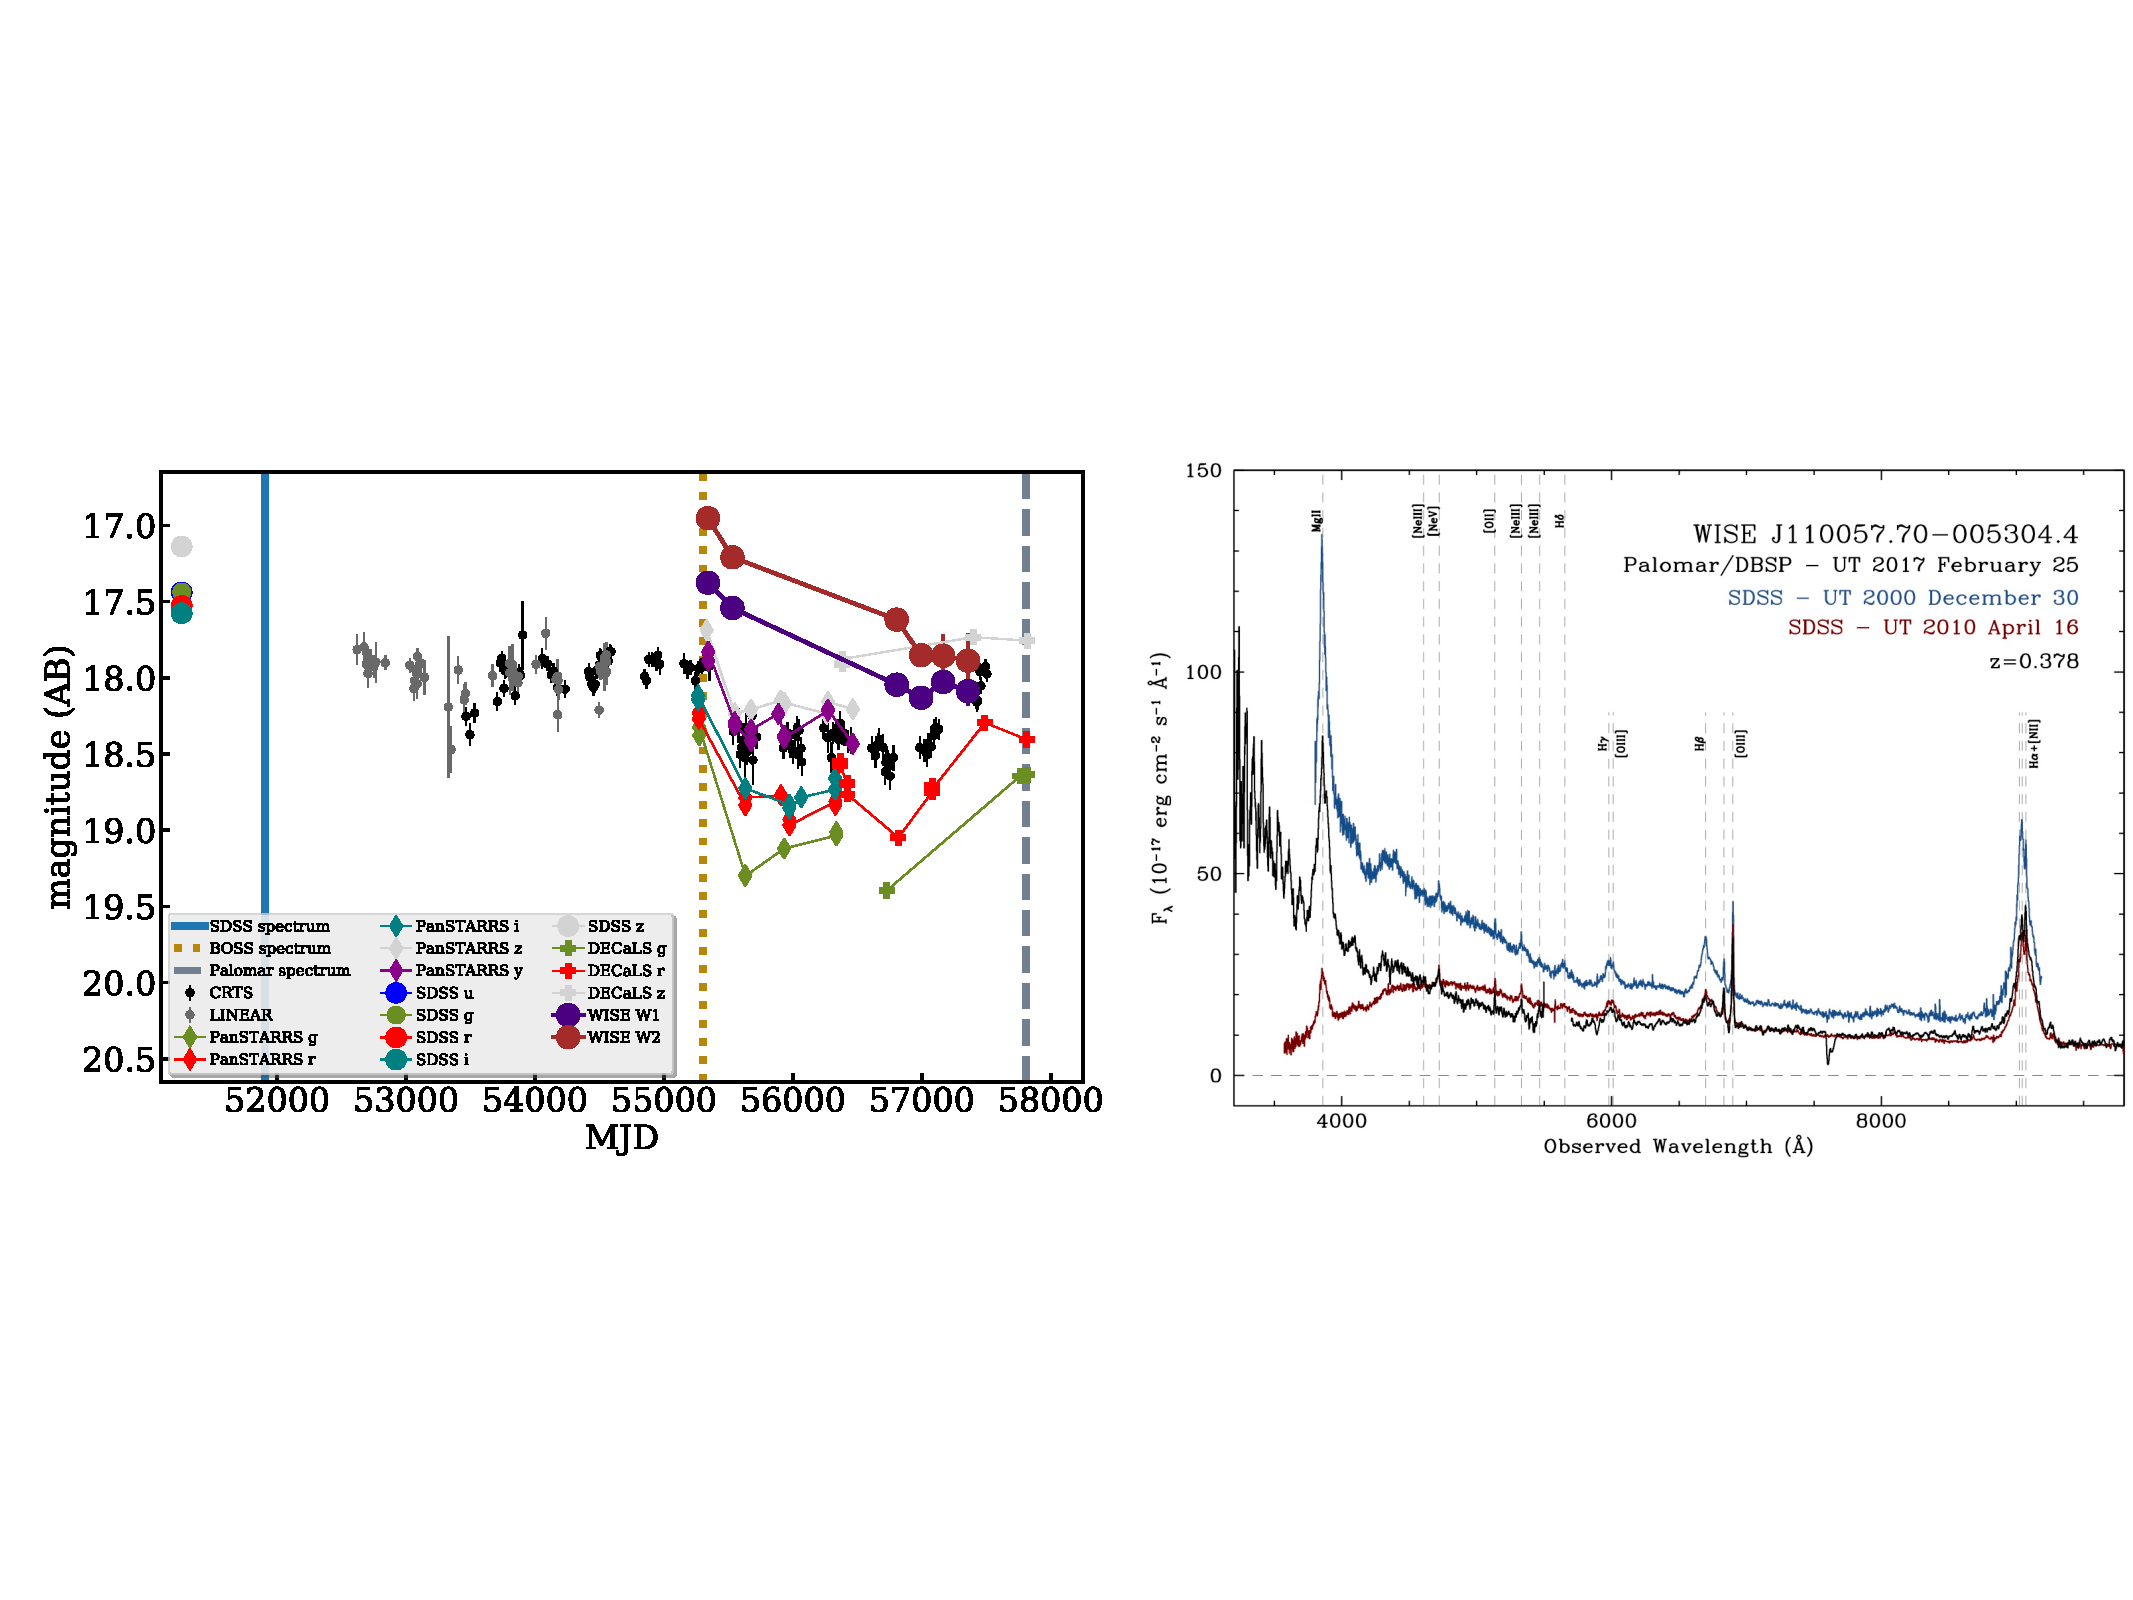
\includegraphics[height=6.25cm,width=17.2cm]
    {figures/J110057_LC_Spectra_20171024.pdf}
    \vspace{-10pt}
    \caption{%\small      
      \footnotesize 
      % \scriptsize
      % \tiny
      {\it (Left:)} The optical and infrared light-curve for J110057; 
      Note the fall in the infrared, whereas there is a decrease, but 
      then recovery in the optical. 
      {\it (Right:)} 
      Three epochs of spectra for J110057. 
      The spectacular downturn in the blue for the 2010 spectrum 
      indicates a dramatic change in the accretion disk.
    }
  \vspace{-16pt}
 \label{fig:J110057}
\end{center}
\end{figure}

%\smallskip \smallskip
\medskip\medskip
\noindent
%{\bf \large \underline{Future Research}}
{\bfseries \large \textsc{\textcolor{Cerulean}{Future Research}}}

\smallskip
\smallskip
\noindent
My future research builds on, and expands my current research program;
I have a bold research vision that is designed to be addressed by a
research group, and the environment, current research areas and
telescope access in the Department of Physics and Astronomy at Dartmouth College
are ideal to
carry out these investigations.
%%
The science questions we seek to address are well-posed, yet strike at
the heart of major and still open extragalactic astrophysical
questions: Do we have a full accounting for the accretion history in
the Universe?  How does the energy `escape' from the central engine to
the host galaxy?  Are the modes of AGN ``feedback'' that regulate a
galaxy the same that regulate the AGN itself?  What are the
star-formation properties of mid-infrared luminous quasars at the peak
of quasar activity?  What are the evolutionary properties, if any, of
dark energy?

\smallskip
\smallskip
\noindent
\textbf{\textsc{New IR investigations into the CLQ Population:}}
Taking advantage of new optical imaging data from the Dark Energy
Camera Legacy Survey \href{http://legacysurvey.org/decamls/}{(DECaLS)}
and new IR light-curves from NEOWISE ([26, 27]), we have made further
in-roads into understanding the CLQ population. This includes
identifying objects with rapidly changing IR light-curves and also
accretion disk changes, e.g. the $z=0.378$ quasar SDSS
J110057-005304.4, see Figure~\ref{fig:J110057}. From J110057, my new
model ([28]) suggests a dramatic new picture of the physics of the
CLQs governed by processes at the innermost stable circular orbit
(ISCO) and the structure of the innermost disk. {\it We have embarked
on a new observation campaign, gaining optical light-curves (from the
Liverpool Telescope) and spectra (from WHT and Palomar) to test this
startling new hypothesis.}

\smallskip
\smallskip
\noindent
%\textbf{\textsc{Extremely Red Quasars: Feedback in action at high-$z$:}}
\textbf{\textsc{Extremely Red Quasars:}}
In [16] I discovered a new class of object, the ``extremely red
quasars'', that have optical spectroscopy from SDSS/BOSS, and
$r-[22\mu{\rm m}]>14$ colors (i.e., $F_{\nu,\, {\rm MIR}} / F_{\nu,\,
{\rm opt}} \gtrsim 1000$) from the Wide-field Infrared Survey Explorer
(WISE; [17]) satellite, see Figure~\ref{fig:ERQ}.  The ERQs are a
unique obscured quasar population with extreme physical conditions
related to powerful outflows across the line-forming regions. These
sources are the signposts of the most dramatic form of quasar feedback
at the peak epoch of galaxy formation, and may represent an active
``blow-out'' phase of quasar evolution ([18], [19]).  However, due to
the current lack of access to mid-infrared spectroscopy, it is still
unknown whether the large IR luminosities observed in these quasars is
from star formation, which would produce strong polycyclic aromatic
hydrocarbon (PAH) spectral features, or, if it is from the hot dust
near the central quasar, which should produce much weaker/no PAH
emission.

\smallskip
\smallskip
\noindent
\textbf{\textsc{SpIES, Telling us about AGN Feedback:}}
My finishing graduate student, John Timlin, is leading the analysis of the {\it
Spitzer}-IRAC Equatorial Survey (SpIES; [20]), which is a new deep
3.6$\mu$m and 4.5$\mu$m imaging survey designed to discover obscured
and faint unobscured quasars in the SDSS Stripe 82 field. The
scientific goals of SpIES are to measure the quasar luminosity
function and clustering to $z\sim4$, and potentially discover a suite
of very high redshift quasars, meanwhile constraining AGN ``feedback''
models.  In [21] we made the first measurements of clustering of
IR-selected $z > 3$ AGNs.  Connecting to current lower-$z$
measurements, we find an ``inefficient feedback'' model is favored,
where all $z>2$ BHs grow to their peak luminosity at $z\sim2$ and then
fully ``shut down'' ($\dot{m}_{\rm accr} \leq 10^{-5}~M_{\odot}$~yr$^{-1}$).

\smallskip \smallskip
\smallskip \smallskip
\noindent
\textbf{\textsc{Early Science with the James Webb Space Telescope: }}
The {\it James Webb Space Telescope} ({\it JWST}) is a 6.5-meter
infrared telescope that will initiate and enable transformative
science. My discovery of the extremely red quasars provides a key
observational clue to the ``major merger'' evolutionary theory for
quasar activity ([29]). I am the P.I. of a large, multi-proposal Cycle 1
programme, that will take maximal advantage of {\it JWST's} new and
uniquely powerful capabilities immediately upon commencing science
operations. The natural science case for {\it JWST} is the detailed
investigation of the incredible richness of the near- and mid-IR spectral
features in the ERQs using the NIRSpec and MIRI spectrographs, and by
utilizing my experience with mid-infrared datasets, surveys and object
discovery, I am leading a team of postdocs and graduate students, to
carry out these investigations. {\it The next JWST Call for Proposals
is in December 2017, and my team is ramping up for a full suite of ERQ
related proposals for this truly revolutionary mission}.


\smallskip
\smallskip
\noindent
\textbf{\textsc{Quasars, Dark Energy and Very Wide Field Surveys: }}
In the community's future is the prospect of very wide-field
ground-based surveys using both imaging and spectroscopy, in the North
and Southern Hemisphere. Building on {\it (i)} my leadership
experience and heritage from being an integral part of BOSS and {\it
(ii)} my world-leading expertise in quasar target selection,
demographics, and physical properties, I will continue to lead the
scientific development of using quasars as large-scale structure (LSS)
tracers in these new surveys.

\smallskip \smallskip
\noindent 
%{\bf \underline {Outline of Future Research:}}
Prior to SDSS-III BOSS, quasars lagged behind massive galaxies as good
tracers of LSS. However, with the evolution of Baryon Acoustic
Oscillation (BAO) and Redshift-Space Distortion (RSD) studies using
BOSS, and in particular the Lyman-$\alpha$ forest (Ly$\alpha$F),
quasars are now seen as key objects in accessing the high-$z$
Universe. Moreover, in the DESI era, there is huge potential to extend
this reach further, first for BAO/RSD and also as Standard Candles. 


\begin{itemize}
\item{{\bf Quasars as Cosmological Probes {\sc I:} Baryon Acoustic
      Oscillations.} I co-led the first investigation that successfully used
    quasars as point test particles to measure the BAO signature
    [15]. This measurement was a cross-correlation with the Ly$\alpha$F,
    but demonstrated that quasars themselves, despite their lower number
    density can trace LSS sufficiently well for BAO studies. This
    provides access to geometry measurements at $z>1$, further
    constraining the Hubble Parameter at high-$z$ and testing the current
    $\Lambda$CDM model.  {\it DESI will be ``the ultimate quasar survey'',
      with sub-per cent measurements of the distance scale (from BAO alone)
      to redshifts of $z\sim3$ using `tracer' and Ly$\alpha$F quasars.}}
  
\item{{\bf Quasars as Cosmological Probes {\sc II:} RSDs with
      Quasars.}  As I proved with the original SDSS sample ([31]), quasars
    can also be used to measure RSDs.  Measurements of the normalized
    growth rate, $f\sigma_{8}$, from RSD using quasars at $z\sim1.5$ is
    crucial since model predictions diverge at these redshifts for
    $\Lambda$CDM+G.R. compared to $f(R)$ gravity, DGP braneworld, and varying
    Gravitational Constant models ([32, 33]). {\it Even with the local
      GW170817 measurements, a range of gravity theories persist and
      testing General Relativity at cosmological scales remains imperative.}}
  
\item{{\bf Quasars as Cosmological Probes {\sc III:} Reverberation
      Mapping Campaigns.}  Recently, [34-37] demonstrated that by using the
    tight relationship between the luminosity of a quasar and the radius
    of its broad-line region, established via reverberation mapping, one
    is able to determine the luminosity distances to quasars.  This means
    that quasars can now be used as standard, or more accurately,
    ``standardizable'' candles (in a very similar way to Type Ia
    supernovae). {\it Thus with light-curve data from LSST and a baseline
      for repeat spectroscopy from SDSS, DESI is ideally placed to exploit
      this new method, with very different systematics to the BAO, and
      access a redshift regime $z>4$ where even the Ly$\alpha$F will not be
      able to offer cosmology constraints.}}

\end{itemize}




\begin{figure}[h]
  \begin{center}
   \hspace{-0.5cm}
%   trim=l b r t
    \includegraphics[height=5.5cm,width=18.0cm] %, trim={0.05cm 0 0.05cm 0},clip]
   {figures/WISE_SDSSzoomHSC_ERQ-image_v3.pdf}
    \vspace{-10pt}
   \caption{%\small   
\footnotesize 
%     \scriptsize
 %    \tiny
The IR and optical imaging of J2323-0100, an archetype of the
``Extremely Red Quasars'' (ERQs) at $z\approx2.5$ and a {\it JWST}
target. Shown are WISE {\it (left)}, where the quasar booms out as
indicated by the arrow; the SDSS image {\it (middle left)} with
zoom-in {\it (middle right)} on the optically faint source, and new
HSC imaging {\it (right)}, which shows tantalizing evidence for a
faint companion galaxy. Optical rest-frame spectra of J2323-0100,
revealed very broad (FWHM = 2500-5000 km s$^{-1}$), strongly
blue-shifted (by up to 1500 km s$^{-1}$) \oiii\ $\lambda$5007\AA\
emission lines in the ERQs. This is suggestive of active outflows and
potentially evidence for AGN feedback in action at the height of SMBH
activity.
}
  \vspace{-12pt}
 \label{fig:ERQ}
\end{center}
\end{figure}





\section{Why Now?}
Figure~\ref{} has the timelines for the major projects that are coming online in the next decade. 


Applicant Principal Investigators 
\subsection{must demonstrate the ground-breaking nature, }
\subsection{ ambition}

\subsection{Feasibility of their scientific proposal.}
%% 
%% Explain the risks of your project and how you plan to address those risks should they materialise.  

WhilteNot risky.  Current data SDSS
I-IV = 520,000 spectra published; 1,000,000 by 2020 (survey ongoing).
PanSTARRS, CRTS, ZTF;

Future:: DESI, ground-based in full construction mode; survey is
starting late 2019) SDSS-V; ground-based; telescope, pipeline,
instrumentation already in place. new surveys start ing 2020 LSST;
ground-based in full construction mode; science survey is starting
2021..)  4MOST; ground-based, in pre construction mode) Euclid, very
muich the most risky programme, since it is space-based, and currently
most likely to slip in schedule. However, although a key ESA facility,
Euclid is arguably the least important of the 5 data streams for our
science case.


\section{Question and Anwer table}
You could also use a two column table having the questions you have set to answer on one side and the respective objectives for each question on the second column (Just a recommendation of the things you could do to make reading your proposal more pleasant for the evaluator).



\newpage
\section{Methodology}

\smallskip
\smallskip
\noindent
Describe your work plan in detail. You can separate the section in terms of work packages/case studies or describe the work in terms of the aims/objectives you described in the previous section, and how you will accomplish those. If you like you can have a flow chart of the different WP’s and how the whole project will come together. Each WP or aims/objectives can be broken down into subtasks.


\begin{itemize}
\item If you have any preliminary results in relation to the work you are describing make sure you emphasise it. Maybe dedicate a separate subsection/heading to preliminary results?
\item You can also list the milestones and the ground breaking features of the planned work. Also how will this WP/aim advance the state of the art in your field? This way even the non-expert evaluator will be able to see the big picture of what you are proposing to do.
\item Describe the balance of your project between the high risk /high gain experiments and what will be the long term benefits in your area from the results you will generate. How will you be advancing the field? In other words emphasise the impact of your work.
\item Have a dedicated section on feasibility of what you are proposing. Explain which WP’s/tasks present high levels of risk. Provide a contingency plan, particularly if any of the tasks are unconventional, present a great challenge and are high risk (but also high gain). Mention your experience and knowledge to hedge against this risk or alternative approaches or help from collaborators. Be “safely adventurous”.
\item Include a gantt chart or a timeline for the evaluators to visualise the timescale of each component of the work you are proposing.
\item Include a 4-5 line summary to recap and remind the evaluator what the essence of the project is and why it so important to get this funded now.
\end{itemize}


\newpage
\section{Resources (including project costs)}
Resources and timelines should entirely reflect the project and nothing else. Link the budget to the proposed activities as accurately as possible.

Feasibility is key.\\
Remember to use whole Euro integers only, when preparing the budget table.
Make sure the numbers on the table match with the numbers on the A forms.
Use this table as it is and don’t reformat it.
Delete all the superscript numbers in final draft to get rid of the text in footer. You will most likely
need the space for your justification.

\input{survey_buyins}

\input{HPC_resources}


\end{document}

